% Section content template for individual Educative lessons
% This file contains the actual content for a specific section
% Generated from Educative API section content

% Section: Final Design of Quora
% Section ID: 6323245837451264
% Section Slug: final-design-of-quora
% Generated: 2025-12-07T22:56:02.238038

\subsection{Limitations of the proposed design}\label{-BoOU68kUn2GwO7n54Bw-}
\\
The proposed design serves all the functional requirements. However, it has a number of serious drawbacks that emerge as we scale. This means that we are unable to fulfill the non-functional requirements. Let's explore the main shortcomings below:

\begin{itemize}
\item
\protect\phantomsection\label{KRUOQtXzhSmVh6AdnXPGE}
\textbf{Limitations of web and application servers}: To entertain the user's request, payloads are transferred between web and application servers, which increases latency because of network I/O between these two types of servers. Even if we achieve parallel computation by separating the web from application servers (that is, the manager and worker processes), the added latency due to an additional network link erodes a user's experience. Apart from data transfer, control communication between the router library with manager and worker processes also imposes additional performance penalties.
\item
\protect\phantomsection\label{ZI6MjziG_3lppjuPpzQk4}
\textbf{In-memory queue failure}: The internal architecture of application servers log tasks and forward them to the in-memory queues, which serve them to the workers. These in-memory queues of different priorities can be subject to failures. For instance, if a queue gets lost, all the tasks in that queue are lost as well, and manual engineering is required to recover those tasks. This greatly reduces the performance of the system. On the other hand, replicating these queues requires increasing RAM size. Also, with the number of features (functional requirements) that our system offers, many tasks can get assembled, which results in insufficient memory. At the same time, it is not desirable to choke application servers with not-so-urgent tasks. For example, application servers should not be burdened with tasks like storing view counts for answers, adding statistics to the database for later analysis, and so on.
\item
\protect\phantomsection\label{s52vsc9CdH3ovLiBh2NpV}
\textbf{Increasing QPS on MySQL}: Because we have a higher number of features offered by our system, few MySQL tables receive a lot of user queries. This results in a higher number of QPS on certain MySQL servers, which can result in higher latency. Furthermore, there is no scheme defined for disaster recovery management in our design.
\item
\protect\phantomsection\label{xi2MNZpowmUvdji63Kou1}
\textbf{Latency of HBase:} Even though HBase allows high real-time throughput, its P99(P99 stands for 99th percentile. It means that 99 percent of the queries are entertained below a specific number. For example, P99 of 20 ms means that 99 percent of the queries will be replied to within 20 ms by a server.) latency is not among the best. A number of Quora features require the ML engine that has a latency of its own. Due to the addition of the higher latency of HBase, the overall performance of the system degrades over time.
\end{itemize}
\\
The issues highlighted above require changes to the earlier proposed design. Therefore, we'll make the following adjustments and update our design:

\begin{figure}[htbp]
 \centering
 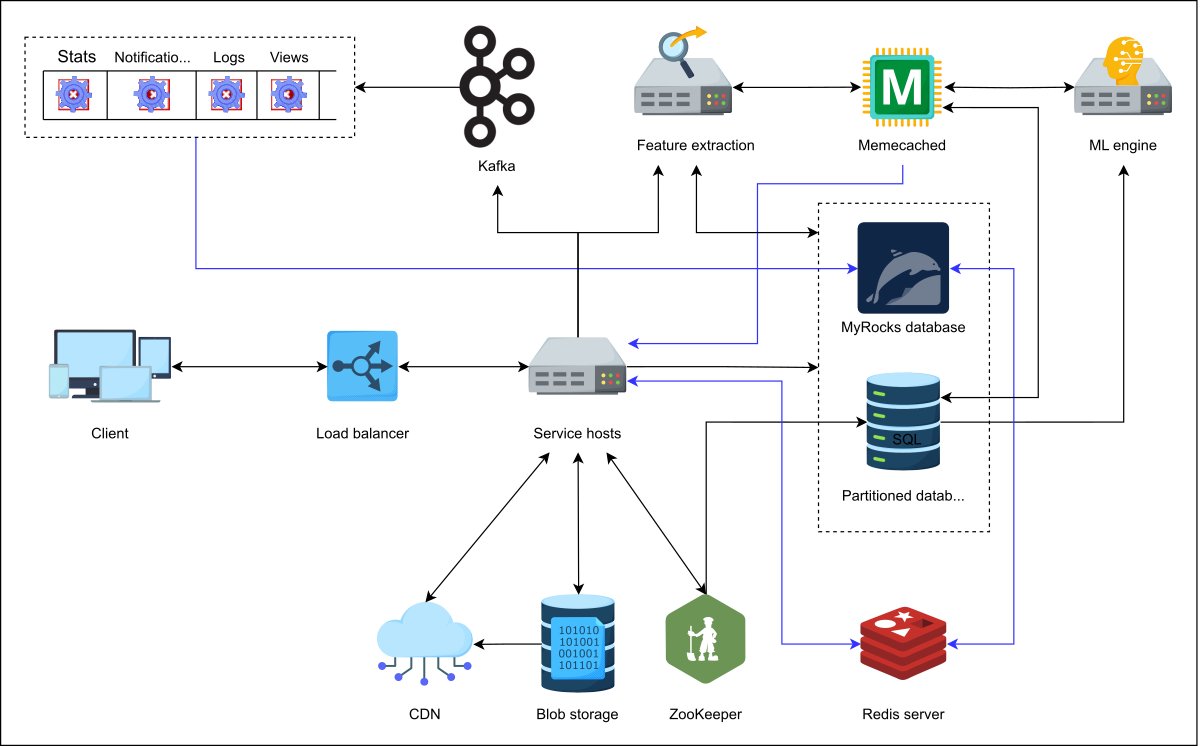
\includegraphics[width=0.5\textwidth]{Images/chapter_27/section_6323245837451264/6720333664354304.png}
 \caption{Detailed design of Quora}
\end{figure}

\subsection{Detailed design of Quora}\label{99AWpuFqqr9APuZHes2Fd}
\\
Let's understand the improvements in our design:

\subsubsection{Service hosts}\label{lqEAXxe0o4b--3-EPuwnK}
\\
We combine the web and application servers within a single powerful machine that can handle all the processes at once. This technique eliminates the network I/O and the latency introduced due to the network hops required between the manager, worker, and routing library processes. The illustration below provides an abstract view of the updated web server architecture:

\begin{figure}[htbp]
 \centering
 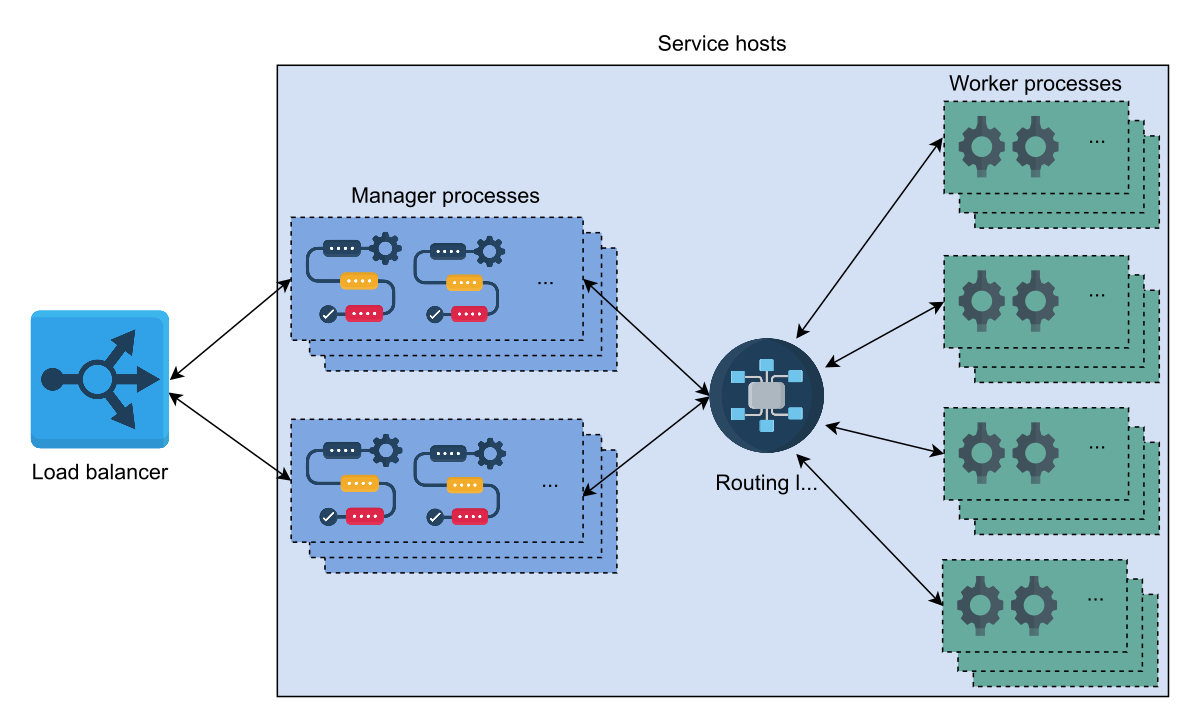
\includegraphics[width=0.5\textwidth]{Images/chapter_27/section_6323245837451264/4576859726282752.png}
 \caption{The updated design, where web and application servers are combined in the service host}
\end{figure}

\subsubsection{Vertical sharding of MySQL}\label{3EhQ9c6rPGuZ6pFZMdcr1}
\\
Tables in the MySQL server are converted to separate shards that we refer to as \textbf{partitions}. A partition has a single primary server and multiple replica servers.
\\
The goal is to improve performance and reduce the load due to an increasing number of queries on a single database table. To achieve that, we do vertical sharding in two ways:

\begin{enumerate}
\item
\protect\phantomsection\label{uqiIWs1taZhWPVN6ADkP6}
We split tables of a single database into multiple partitions. The concept is depicted in Partitions 2 and 3, which embed Tables 4 and 3, respectively.
\item
\protect\phantomsection\label{_wWbLn-dbmAa3Tu1ca_ud}
We combine multiple tables into a single partition, where \texttt{join} operations are anticipated. The concept is depicted in Partition 1, which embeds Tables 1 and 2.
\end{enumerate}
\\
Therefore, we are able to co-locate related data and reduce traffic on hot data. The illustration below depicts vertical sharding at Quora.

\begin{figure}[htbp]
 \centering
 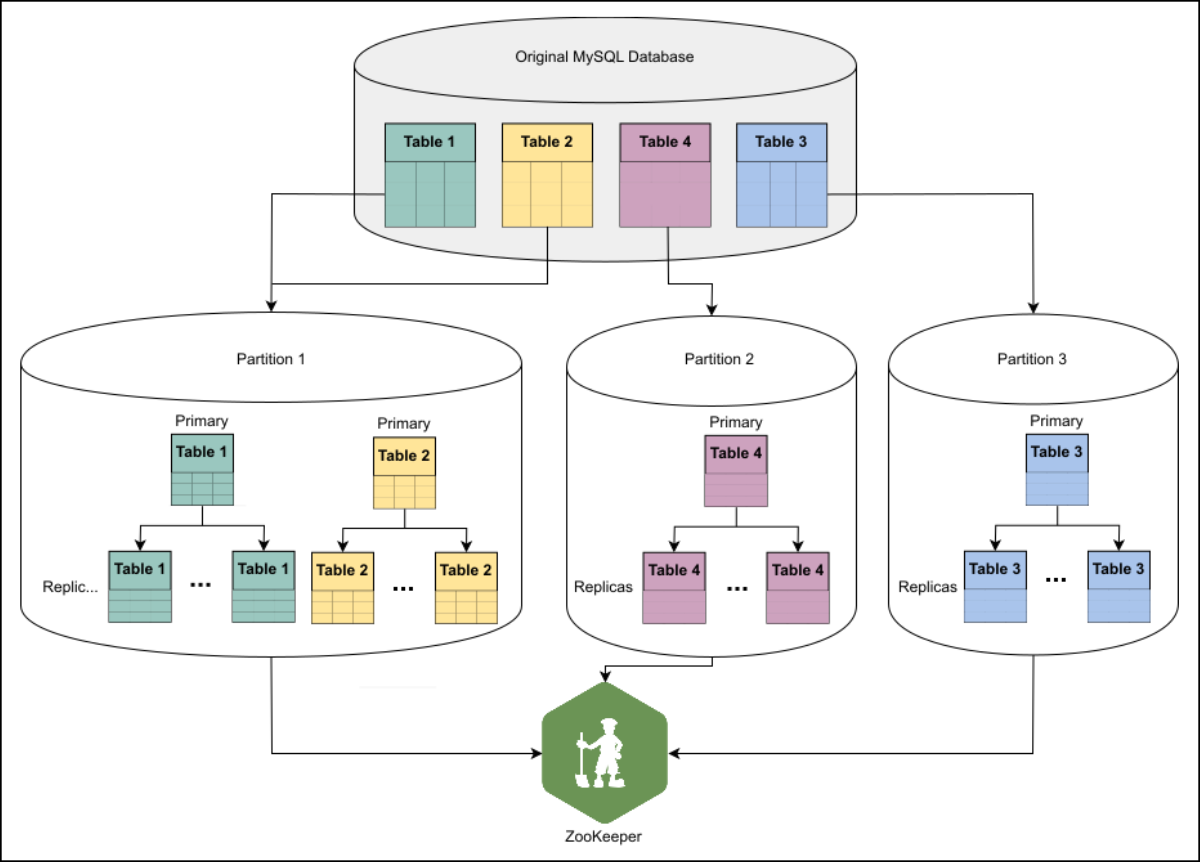
\includegraphics[width=0.5\textwidth]{Images/chapter_27/section_6323245837451264/5219262516166656.png}
 \caption{The architecture of vertical sharding at Quora}
\end{figure}

After we complete the partitioning, we require two types of mappings or metadata to complete our scaling process:

\begin{enumerate}
\item
\protect\phantomsection\label{5tgXI4x6wMRDRoul3kQ19}
Which partitions contain which tables and columns?
\item
\protect\phantomsection\label{y5ltaGZix4Tth6WJWDK1N}
Which hosts are primary and replicas of a particular partition?
\end{enumerate}
\\
Both of these mappings are maintained by a service like ZooKeeper.
\\
The sharded design above ensures scalability because we are able to locate related data in a single partition, and therefore it eliminates the need for querying data from multiple shards. Also , the number of read-replicas can be increased for hot shards, or further sharding may be performed. For edge cases where joining may be needed, we can perform it at the application level.
\begin{quote}
\textbf{Note:} Vertical sharding is of particular interest in Quora's design because horizontal sharding is more common in the database community. The main idea behind vertical sharding is to achieve scalability by carefully dividing or re-locating tables and eliminating join operations across different shards. Nevertheless, a vertically sharded partition or table can grow horizontally to an extent where horizontal sharding will be necessary to retain acceptable performance.
\end{quote}
\subsubsection{MyRocks}\label{udep9t9y8bH0VP9Hv7luZ}
\\
The new design embeds MyRocks as the key-value store instead of HBase. We use the MyRocks version of RocksDB for two main reasons:

\begin{enumerate}
\item
\protect\phantomsection\label{vtcO16N2ofS2V6SEmnbW1}
MyRocks has a lower p99 latency instead of HBase. Quora claims to have reduced P99 latency from 80 ms to 4 ms using MyRocks.
\item
\protect\phantomsection\label{hg5zyalX_8HeLUkuSnya1}
There are operational tools that can transfer data between MyRocks and MySQL.
\end{enumerate}
\begin{quote}
\textbf{Note:} Quora serves the ML compute engine by extracting features from questions and answers stored in MySQL. In this case, the operational tools come in handy to transfer data between MyRocks and MySQL.
\end{quote}
\subsubsection{Kafka}\label{gfNnDl0nfEgMlUzldnwm5}
\\
Our updated design reduces the request load on service hosts by separating not-so-urgent tasks from the regular API calls. For this purpose, we use Kafka, which can disseminate jobs among various queues for tasks such as the view counter (see \href{https://www.educative.io/courses/grokking-the-system-design-interview/system-design-the-sharded-counters}{Sharded Counters}), notification system, analytics, and highlight topics to the user. Each of these jobs is executed through cron jobs(It is also called ``cron,'' and is a command-line utility that is used to schedule tasks on UNIX-like operating systems.).

\subsubsection{Technology usage}\label{gQHazwEVepuuGW6Xq_fuB}
\\
Services that scale quickly have little time to develop new features and handle an increasing number of requests from users. Such services employ cloud infrastructure to handle spikes in traffic. Also, the choice of programming language is important. Just like we mentioned that YouTube chose Python for faster programming, we can apply the same logic to Quora. In fact, Quora uses the Python Paste web framework.
\\
It is desirable to use a faster programming language like C++ to develop the feature extraction service(Quora refers to their feature extraction service as Alchemy, a scalable and high-performance tool.). For online recommendation services through a ML engine, feature extraction service should be quick, to enable the ML engine to accomplish accurate recommendations. Not only that, but reducing the latency burden on the ML engine allows it to provide a larger set of services. We can employ the Thrift service to support interoperability between programming languages within different components.
\\
Features like comments, upvotes, and downvotes require frequent page updates from the client side. \textbf{Polling} is a technique where the client (browser) frequently requests the server for new updates. The server may or may not have any updates but still responds to the client. Therefore, the server may get uselessly overburdened. To resolve this issue, Quora uses a technique called \textbf{long polling}, where if a client requests for an update, the server may not respond for as long as 60 seconds if there are no updates. However, if there is an update, the server will reply immediately and allow the client to make new requests.

\begin{figure}[htbp]
 \centering
 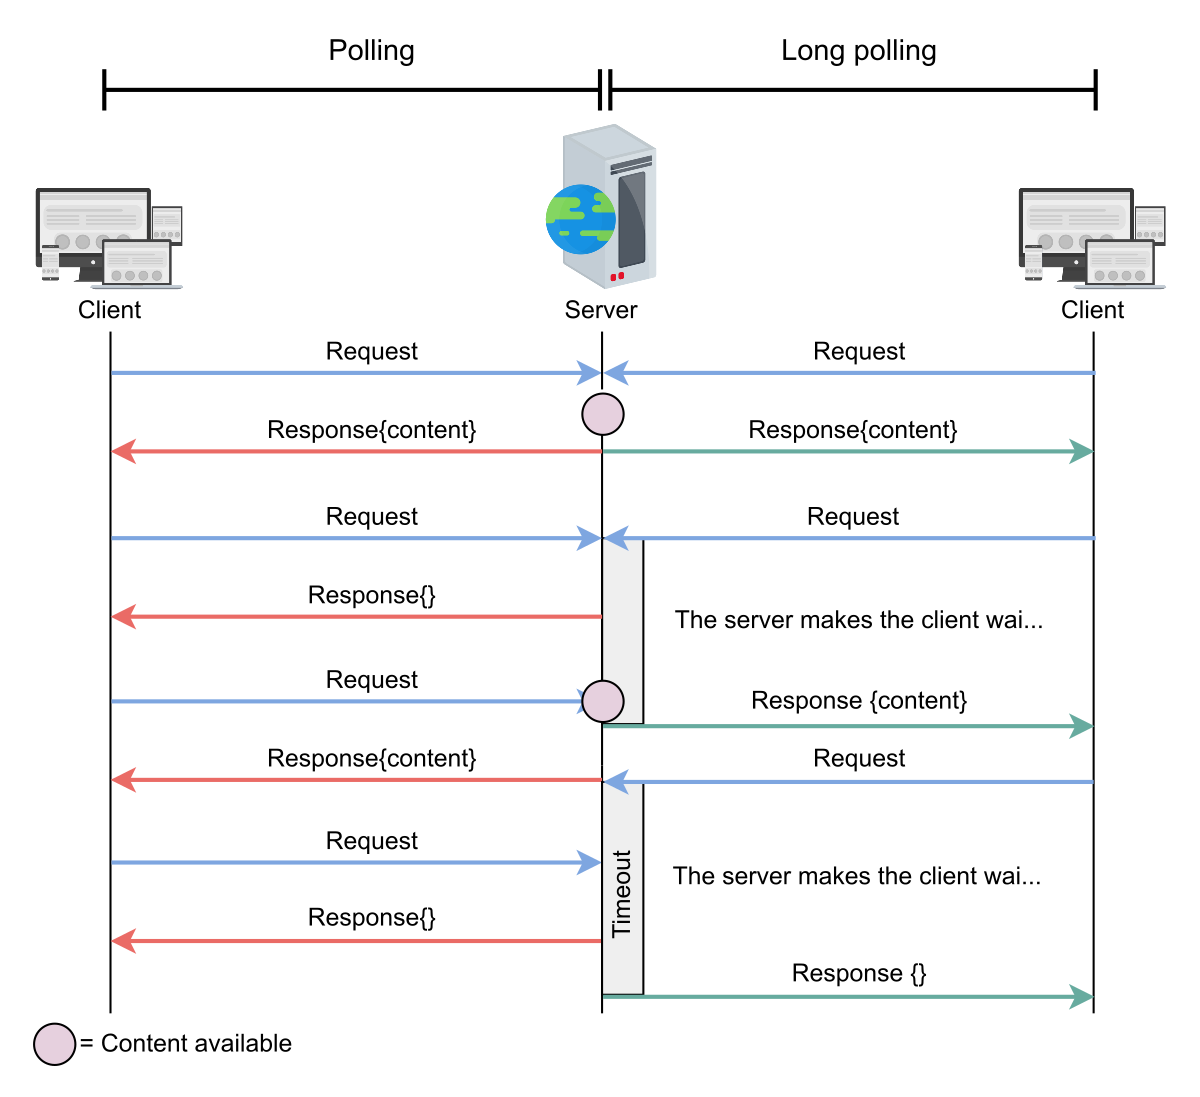
\includegraphics[width=0.5\textwidth]{Images/chapter_27/section_6323245837451264/6502274138636288.png}
 \caption{Polling vs. long polling}
\end{figure}

Lastly, Memcached can employ \texttt{multiget()} to obtain multiple keys from the cache shards to reduce the retrieval latency of multiple keys.
\begin{quote}
\textbf{Note:} Quora has employed AWS to set up a good number of its infrastructure elements, including S3 (see the \href{https://www.educative.io/courses/grokking-the-system-design-interview/system-design-a-blob-store}{Blob Storage chapter}) and Redshift(Redshift is a data warehouse product from Amazon that is based on PostgreSQL. It can handle complex queries, allowing large-scale data transfer. Quora uses Redshift to store view counters.) storage.
\end{quote}

\begin{quote}
\textbf{Quiz:}
\textbf{Question 1:} What would be considered a good approach for communication between different manager and worker processes within the service hosts?
\textbf{Answer:} Two approaches are feasible for communication: 1. UNIX sockets 2. TCP

connections Sockets (Unix or TCP) allow data streaming between sender and receiver with appropriate flow control (and congestion control in the case of TCP). That means the sender and receiver can send variable-size data in a decoupled fashion. Other interprocess communication techniques like shared memory may not be feasible because they require estimating the size of the required memory segment, which makes the participants more coupled. Also, it will not work across physical servers. So, we prefer sockets due to their high decoupling, flow control, and ability to work for both single servers or over the network.
\textbf{Question 2:} In our detailed design, we have employed Kafka to handle our view counter of answers. Why do you think we made this decision?
\textbf{Answer:} Depending on the topic label, many users can view the response to a question at once. This can choke the servers. Instantaneous update of the view counter is also not an important product feature. Therefore,

Kafka is suitable for handling these tasks. Quora handles these tasks in two minutes or less. Nonetheless, we can use sharded counters as an effective solution to the view counter problem.
\textbf{Question 3:} What is the main advantage of using long polling instead of polling?
\textbf{Answer:} Long polling transfers the control to the server side instead of the client, which has no information about the updates in content. If the server is in control, it can reply as soon as there is fresh content. As a result, it reduces the request load on itself. However, long polling is a resource-intensive solution because it keeps the connection persistent or alive for a longer period of time. WebSockets are another low-latency solution with low overhead. However, WebSockets might be an overkill for the features offered by Quora.
\end{quote}



% End of section content